\chapter{Background and Related Work}
\label{chap:related_work}

\section{Foundational Knowledge}
\label{sec:foundational_knowledge}

\subsection{Visually Rich Documents (VRDs) and OCR Pipelines}
\label{subsec:vrd_ocr}

A \textbf{Visually Rich Document (VRD)} is any document whose semantic interpretation is jointly determined by its textual words, its two-dimensional spatial layout, and its visual styling~\cite{cui2021documentai}. Typical examples include tax forms, commercial invoices, point-of-sale (POS) receipts, identity cards, financial tables, and academic articles.

In practical Document AI pipelines, processing a VRD image $\mathbf{I} \in \mathbb{R}^{H \times W \times 3}$ begins with an \textbf{Optical Character Recognition (OCR)} stage (e.g., Tesseract, EasyOCR, PaddleOCR, or commercial cloud OCR engines) that performs two sub-tasks:
\begin{enumerate}
    \item \textbf{Text Detection:} Localizes text regions at both the word level and the text-line (segment) level, outputting axis-aligned bounding boxes $\tilde{\mathbf{b}}_i = (\tilde{x}_0^{(i)}, \tilde{y}_0^{(i)}, \tilde{x}_1^{(i)}, \tilde{y}_1^{(i)})$.
    \item \textbf{Text Recognition:} Transcribes the cropped image region of each detected box into a sequence of characters or words $w_i$, along with hierarchical grouping indices $s_i$ that indicate which words belong to the same contiguous text line or block.
\end{enumerate}

Because scanned documents vary widely in pixel resolution $(W, H)$, feeding raw pixel coordinates directly into neural networks causes scale variance. Standard multi-modal document models normalize all coordinates into a discrete integer grid $[0, 1000] \times [0, 1000]$, ensuring scale invariance across arbitrary aspect ratios.

\subsection{Sequence Labeling and the BIO/IOB2 Tagging Scheme}
\label{subsec:iob2_scheme}

To extract multi-word semantic entities (such as a customer's full address or a multi-word menu item) using token-level classification, KIE benchmarks adopt the \textbf{IOB2 (Inside--Outside--Beginning)} tagging convention~\cite{ramshaw1995text}. Given $K$ semantic entity categories $\mathcal{E} = \{e_1, \dots, e_K\}$, each subword token $w_i$ is assigned a label $y_i \in \mathcal{Y}$ according to three rules:
\begin{itemize}
    \item $\texttt{B-}e_k$ (\textit{Beginning}): Assigned to the very first token of an entity mention belonging to category $e_k$.
    \item $\texttt{I-}e_k$ (\textit{Inside}): Assigned to all subsequent tokens inside the same entity mention of category $e_k$.
    \item $\texttt{O}$ (\textit{Outside}): Assigned to background tokens that do not belong to any target entity.
\end{itemize}

When a word is split into $m > 1$ subword tokens $(w_{i,1}, w_{i,2}, \dots, w_{i,m})$ by Byte-Pair Encoding (BPE)~\cite{sennrich2016neural,liu2019roberta}, standard evaluation protocols assign the ground-truth label $y_i$ to the first subword $w_{i,1}$ and mask out the remaining subwords $(w_{i,2}, \dots, w_{i,m})$ with the ignore index $-100$ during loss computation and metric evaluation, or propagate predictions consistently at the word/span level.

\subsection{Transformer Architecture and Multi-Head Self-Attention}
\label{subsec:transformer_attention}

The \textbf{Transformer} architecture~\cite{vaswani2017attention} forms the computational backbone of modern pre-trained language and vision-language models~\cite{devlin2019bert,liu2019roberta,dosovitskiy2020image}. Given an input hidden matrix $\mathbf{H} \in \mathbb{R}^{N \times d}$ of sequence length $N$ and hidden dimension $d$, a \textbf{Multi-Head Self-Attention (MHSA)} layer projects $\mathbf{H}$ into query ($\mathbf{Q}$), key ($\mathbf{K}$), and value ($\mathbf{V}$) subspaces across $H_{\text{head}}$ parallel attention heads, each of dimension $d_k = d / H_{\text{head}}$:
\begin{equation}
    \mathbf{Q}_h = \mathbf{H}\mathbf{W}_h^Q, \quad
    \mathbf{K}_h = \mathbf{H}\mathbf{W}_h^K, \quad
    \mathbf{V}_h = \mathbf{H}\mathbf{W}_h^V, \quad h \in \{1, \dots, H_{\text{head}}\},
\end{equation}
where $\mathbf{W}_h^Q, \mathbf{W}_h^K, \mathbf{W}_h^V \in \mathbb{R}^{d \times d_k}$ are learnable projection matrices. The scaled dot-product attention for head $h$ is computed as:
\begin{equation}
    \text{Attention}(\mathbf{Q}_h, \mathbf{K}_h, \mathbf{V}_h) = \text{softmax}\!\left(\frac{\mathbf{Q}_h \mathbf{K}_h^\top}{\sqrt{d_k}} + \mathbf{B}_{\text{rel}}\right)\mathbf{V}_h,
    \label{eq:scaled_dot_attention}
\end{equation}
where $\mathbf{B}_{\text{rel}} \in \mathbb{R}^{N \times N}$ denotes optional 1D and 2D relative position bias matrices injected into the attention logits. The outputs of all $H_{\text{head}}$ heads are concatenated and projected via $\mathbf{W}^O \in \mathbb{R}^{d \times d}$, followed by residual connections, Layer Normalization (\texttt{LayerNorm}), and a position-wise Feed-Forward Network (\texttt{FFN}) with GELU activation.

\section{Evolution of the LayoutLM Model Family}
\label{sec:layoutlm_evolution}

\subsection{LayoutLM (v1) and LayoutLMv2}
\label{subsec:layoutlm_v1_v2}

\textbf{LayoutLM}~\cite{xu2020layoutlm} pioneered joint pre-training of text and layout by augmenting BERT~\cite{devlin2019bert} with 2D spatial coordinate embeddings $(x_0, y_0, x_1, y_1)$ and training on 11 million scanned documents from the IIT-CDIP collection using Masked Visual-Language Modeling (MVLM). However, LayoutLM (v1) only injected visual region features from a Faster R-CNN backbone during downstream fine-tuning rather than during pre-training.

\textbf{LayoutLMv2}~\cite{xu2021layoutlmv2} integrated visual features directly into pre-training using a ResNeXt-FPN convolutional backbone and introduced \textbf{Spatial-Aware Self-Attention}, adding learnable 1D and 2D relative position biases $\mathbf{B}_{\text{rel}}^{(1\text{D})}$, $\mathbf{B}_{\text{rel}}^{(2\text{D}_x)}$, and $\mathbf{B}_{\text{rel}}^{(2\text{D}_y)}$ to the self-attention mechanism (Equation~\ref{eq:scaled_dot_attention}). Despite strong accuracy gains, LayoutLMv2 suffered from a heavy CNN visual backbone bottleneck and required complex region-level supervision.

\subsection{LayoutLMv3: Unified Text-Layout-Image Pre-Training}
\label{subsec:layoutlmv3_backbone}

\textbf{LayoutLMv3}~\cite{huang2022layoutlmv3} represents a major paradigm shift by eliminating heavy CNN backbones entirely and adopting a unified multimodal Transformer inspired by Vision Transformers (ViT)~\cite{dosovitskiy2020image} and BEiT~\cite{bao2021beit}. Figure~\ref{fig:layoutlmv3_arch} illustrates the overall pre-training and representation architecture of LayoutLMv3.

\begin{figure}[htbp]
    \centering
    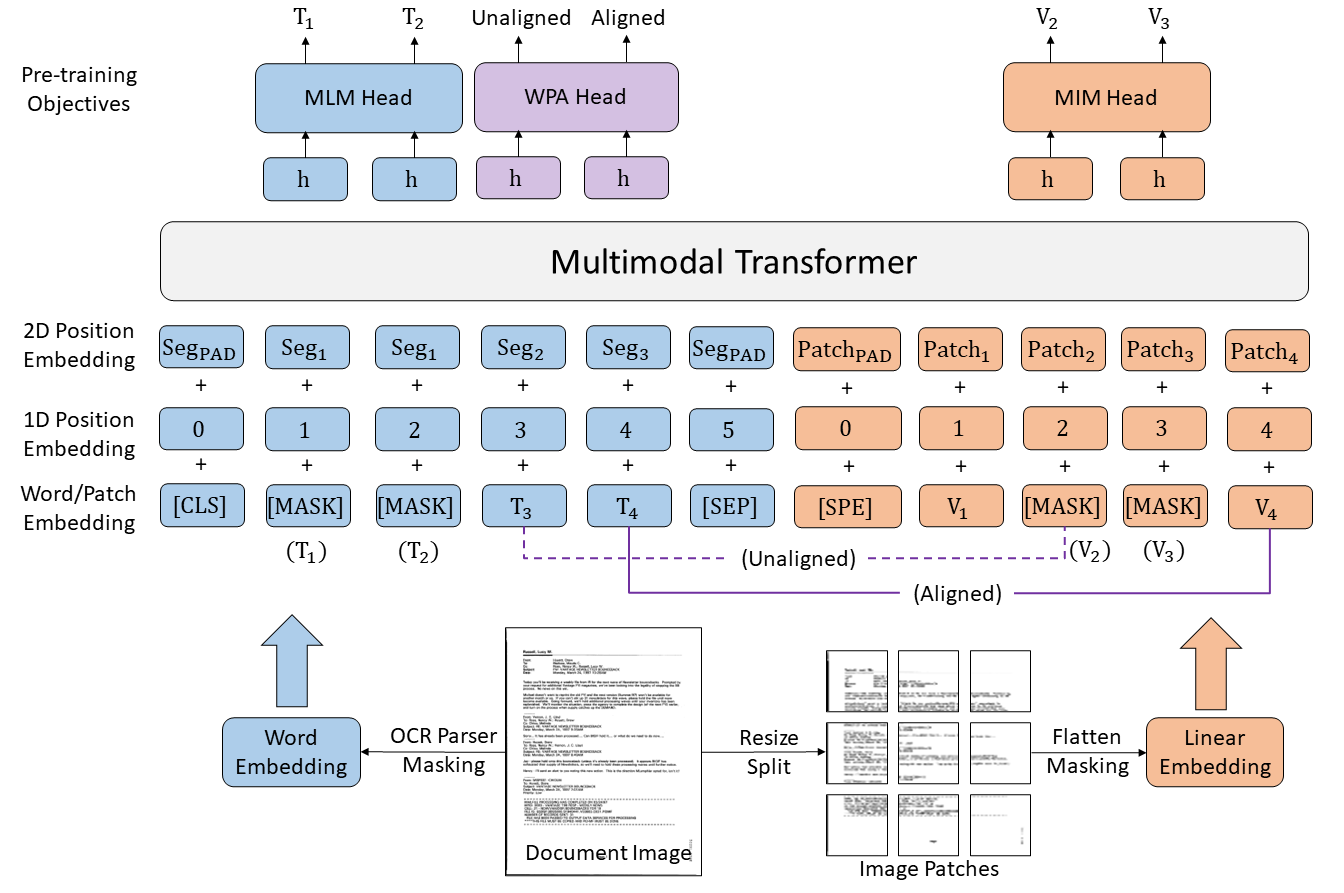
\includegraphics[width=0.92\textwidth]{chapter2/architecture.png}
    \caption{Overview of the unified multimodal LayoutLMv3 architecture combining word-patch alignment, masked language modeling, and masked image modeling~\cite{huang2022layoutlmv3}.}
    \label{fig:layoutlmv3_arch}
\end{figure}

In LayoutLMv3, the multimodal input sequence fed into the Transformer encoder consists of two concatenated streams:
\begin{enumerate}
    \item \textbf{Text + 2D Layout Stream ($\mathbf{E}^{\text{text}} \in \mathbb{R}^{L \times d}$):}
    Text sequences are tokenized via RoBERTa BPE~\cite{liu2019roberta}. Crucially, instead of assigning noisy word-level bounding boxes to every token, LayoutLMv3 assigns \textbf{segment-level (line-level) bounding boxes} to all words belonging to the same visual text segment, reducing OCR box jitter. For the $i$-th token, its unified text-layout embedding $\mathbf{e}_i^{\text{text}} \in \mathbb{R}^d$ is the sum of its word embedding, 1D position embedding, token-type embedding, and 2D spatial layout embedding:
    \begin{equation}
        \mathbf{e}_i^{\text{text}} = \text{LN}\!\left( \mathbf{e}^{\text{word}}(w_i) + \mathbf{e}^{\text{pos1D}}(i) + \mathbf{e}^{\text{type}}(0) + \mathbf{e}^{\text{pos2D}}(\mathbf{b}_i) \right).
        \label{eq:layoutlmv3_text_emb}
    \end{equation}

    \item \textbf{Visual Patch Stream ($\mathbf{E}^{\text{image}} \in \mathbb{R}^{(M+1) \times d}$):}
    The document image $\mathbf{I} \in \mathbb{R}^{H_{\text{img}} \times W_{\text{img}} \times 3}$ (typically $224 \times 224$) is partitioned into $M = (H_{\text{img}}/P) \times (W_{\text{img}}/P)$ non-overlapping patches of size $P \times P$ ($P=16$, yielding $M = 14 \times 14 = 196$ patches), linearly projected to dimension $d$ with a prepended visual class token $[\texttt{CLS}_{\text{vis}}]$ and 1D visual position embeddings (total length $M+1 = 197$).
\end{enumerate}

LayoutLMv3 is pre-trained jointly with three self-supervised objectives:
\begin{itemize}
    \item \textbf{Masked Language Modeling (MLM):} Reconstructs $30\%$ of text tokens masked via span masking conditioned on unmasked text and visual patches.
    \item \textbf{Masked Image Modeling (MIM):} Reconstructs $40\%$ of visual patches masked via blockwise masking by predicting discrete visual tokens generated by a latent dVAE tokenizer~\cite{bao2022beit}.
    \item \textbf{Word-Patch Alignment (WPA):} Predicts via binary classification whether the visual patch corresponding to each unmasked text token is also unmasked or masked, enforcing fine-grained cross-modal alignment between text tokens and spatial image regions.
\end{itemize}

\section{Related Work on Structural Document Intelligence and KIE}
\label{sec:related_work_kie}

Key Information Extraction from visually rich documents has rapidly evolved from early pipeline architectures to multimodal foundation models and structural inductive biases. In this section, we examine recent breakthroughs across five tightly related research frontiers:

\subsection{Multimodal Foundation Transformers in Document AI}
The transition from text-only language models to visually rich document intelligence was pioneered by LayoutLM~\cite{xu2020layoutlm}, which augmented BERT~\cite{devlin2019bert} with 2D coordinate embeddings. LayoutLMv2~\cite{xu2021layoutlmv2} and DocFormer~\cite{appalaraju2021docformer} incorporated CNN-based visual features via spatial-aware cross-attention. LayoutLMv3~\cite{huang2022layoutlmv3} further streamlined document pre-training by eliminating heavy CNN feature extractors in favor of linear image patch embeddings~\cite{kim2021vilt,li2022dit}, coupled with unified MLM, MIM, and WPA objectives. Meanwhile, LiLT~\cite{wang2022lilt} explored language-independent layout representation by learning dual-stream text and geometry interactions, and UniDoc~\cite{gu2021unidoc} introduced unified contrastive multimodal pre-training.

\subsection{Structural Modeling, Graph Networks, and Reading-Order Pipelines}
Standard 2D bounding boxes treat spatial coordinates as flat values, omitting hierarchical grouping. StructuralLM~\cite{li2021structurallm} introduced cell-level 2D positions to bridge word and block representations. BROS~\cite{hong2022bros} explicitly encoded relative spatial bounding box offsets and angular orientations to handle complex reading orders. FormNet~\cite{lee2022formnet} and USTC-iFLYTEK~\cite{ustciflytek2023} utilized graph convolutional and attention networks to reconstruct semantic links across non-sequential form entities. GraphLayoutLM~\cite{li2023graphlayoutlm} explicitly injected layout graphs into self-attention. More recently, ROAP~\cite{xie2026roap} integrated adaptive XY-cut gap algorithms and attention priors to enforce reading-order constraints directly within LayoutLMv3, demonstrating the crucial importance of structural ordering in KIE.

\subsection{Recent Architectural Enhancements on LayoutLMv3}
Due to its parameter efficiency and strong baseline representations, LayoutLMv3 has become the premier foundation backbone for downstream structural enhancements. AETNet~\cite{aetnet2023} introduced cross-modal alignment enhancement modules and auxiliary contrastive losses to tighten visual-lexical binding. OTCR~\cite{otcr2026} framed cross-modal feature routing through optimal transport theory, dynamically routing salient visual cues to corresponding text tokens. DocExtractNet~\cite{docextractnet2024} incorporated P-Tuning precision hints alongside dual-branch image enhancement to stabilize entity boundaries on degraded document scans. Our proposed architecture advances this research direction by introducing explicit Hierarchical Position Encoding (HPE), a lightweight ReZero-gated Segment Context Module (SCM), and Intra-Line Boundary Loss.

\subsection{Generative LLMs vs. Discriminative Sequence Labeling}
With the rise of Large Language Models (LLMs), generative Document AI models such as DONUT~\cite{kim2022donut}, DocLLM~\cite{wang2024docllm}, LayoutLLM~\cite{luo2024layoutllm}, LayTextLLM~\cite{laytextllm2024}, and DocLayLLM~\cite{doclayllm2024} formulate KIE as autoregressive text generation. While LLM-based approaches demonstrate impressive zero-shot reasoning, they incur prohibitive computational inference costs and struggle with precise spatial grounding back to OCR coordinates~\cite{wang2024docllm}. Concurrently, in-context learning pipelines like SAIL~\cite{sail2024} and generative error correctors like GENKIE~\cite{genkie2023} explore training-free prompting. To bridge this trade-off, hybrid discriminative frameworks such as P2Net~\cite{p2net2025} and PM3-KIE~\cite{pm3kie2025} combine frozen representations with parallel prediction matrices and probabilistic reasoning layers. For high-throughput enterprise pipelines requiring microsecond latency and exact bounding-box verification, lightweight discriminative sequence-labeling models with structural inductive biases remain exceptionally compelling.

\subsection{Relation Extraction and Parameter Adaptation}
In the broader scope of Information Extraction and continual learning, researchers have focused on prototype augmentation and structural parameter adaptation. Pham Thi et al.~\cite{phamthi2022memory} demonstrated that memory-based prototype regularization substantially preserves semantic entity boundaries and prevents catastrophic forgetting in relation extraction. Furthermore, Pham Thi et al.~\cite{phamthi2025dakta} developed directional Kolmogorov-Arnold task arithmetic to regularize sub-network updates. These principles provide valuable motivation for stabilizing sub-network updates and maintaining parameter efficiency when fine-tuning multimodal Transformers.

Table~\ref{tab:related_work_comparison} summarizes the architectural characteristics of representative Document AI models compared with our proposed Structure-Aware LayoutLMv3 framework.

\begin{table}[htbp]
\centering
\small
\caption{Architectural comparison between existing KIE models and our proposed Structure-Aware LayoutLMv3.}
\label{tab:related_work_comparison}
\renewcommand{\arraystretch}{1.25}
\setlength{\tabcolsep}{2.5pt}
\begin{tabularx}{\textwidth}{|>{\RaggedRight\arraybackslash}p{3.2cm}|>{\Centering\arraybackslash}p{2.2cm}|>{\Centering\arraybackslash}p{3.2cm}|C|C|C|}
\hline
\makecell{\textbf{Model /}\\\textbf{Method}} & \makecell{\textbf{Visual}\\\textbf{Backbone}} & \makecell{\textbf{2D Position}\\\textbf{Encoding}} & \makecell{\textbf{Segment}\\\textbf{Attention}} & \makecell{\textbf{ReZero}\\\textbf{Gate}} & \makecell{\textbf{Boundary}\\\textbf{Loss}} \\ \hline
\makecell[l]{BERT~\cite{devlin2019bert}~/\\ \relax RoBERTa~\cite{liu2019roberta}} & \makecell{None\\(Text Only)} & \makecell{None\\(1D Only)} & No & No & No \\ \hline
\makecell[l]{LayoutLM (v1)\\\mbox{\cite{xu2020layoutlm}}} & \makecell{Faster\\R-CNN} & \makecell{Isotropic\\Word Box} & No & No & No \\ \hline
\makecell[l]{LayoutLMv2\\\mbox{\cite{xu2021layoutlmv2}}} & \makecell{ResNeXt-\\FPN} & \makecell{Isotropic\\Word Box} & No & No & No \\ \hline
\makecell[l]{StructuralLM\\\mbox{\cite{li2021structurallm}}} & None & \makecell{Cell-Level\\2D Box} & \makecell{Cell-\\Level} & No & No \\ \hline
\makecell[l]{Baseline\\\mbox{LayoutLMv3}~\cite{huang2022layoutlmv3}} & \makecell{Linear\\Patch} & \makecell{Isotropic\\($d/6$)} & \makecell{Shared\\Box} & No & No \\ \hline
\makecell[l]{\textbf{Ours}\\\textbf{(Structure-}\\\textbf{Aware}\\\textbf{\mbox{LayoutLMv3})}} & \makecell{\textbf{Linear}\\\textbf{Patch}} & \makecell{\textbf{Hierarchical}\\\textbf{HPE ($d_x \neq d_y$)}} & \makecell{\textbf{Yes}\\(SCM)} & \makecell{\textbf{Yes}\\($\alpha$ Gate)} & \makecell{\textbf{Yes}\\($\mathcal{L}_{\text{bound}}$)} \\ \hline
\end{tabularx}
\end{table}

As highlighted in Table~\ref{tab:related_work_comparison}, while baseline LayoutLMv3 shares segment bounding boxes across words in the same line, it lacks asymmetric axis encoding, explicit segment-level consensus attention, and intra-line boundary regularization—precisely the three innovations developed in Chapter~\ref{chap:methodology}.

